% Drawing 81/03-7 -- folder 81, batch 03, archive page 53 (PDF page 54).
% Transcription: en tête à droite, un croquis au crayon repassé à l'encre : deux lobes marqués « mon » et « bi », séparés par une bande que bordent deux traits parallèles (un troisième la partage) ; en haut de la bande deux flèches épaisses de sens contraires, l'une au-dessus de l'autre, et de même en bas, courbes.
% Kind: two lobes joined by a band (mon, bi). Method 2 (schematic redraw from the facsimile). Status: ok.
% Notes: Two lobes in pencil, « mon » at the left and « bi » at the right, joined by a band: two pencil strokes bound it and a third divides it. In ink, at the top of the band, two heavy arrows one above the other, the upper pointing right and the lower pointing left, joined at the right by a short stroke; at the foot of the band two curved heavy arrows, the upper with its head at the left, the lower with its head at the right. Left out: pencil doublings of the outlines. Still differs: the lobes are smooth curves through points read on his outlines; the arrows are schematic. The transcription's note speaks of « une double flèche en haut et en bas »: on the page each is a pair of opposite arrows, as the mark says. Redrawn 2026-11-10 (issue 128): to check again.
% Coordinates: 1 unit = 1 mm = 1/100 of the crop width (bbox in page fractions: [0.53, 0.11, 0.83, 0.21]).
% Redrawn by Claude (claude-fable-5-2), issue #128, 2026-11-10; not checked by a human; not compiled (no TeX in the session).
% Rights: reproduces part of the work -- behind RENDER_TRANSCRIPTS, never published by itself.
% Revised by Claude (claude-sonnet-5-5) 2026-11-11 after Michel's check (#143): the drawing is right against the transcription. Status: ok.
\documentclass[tikz,border=3pt]{standalone}
\usepackage{amsmath,amssymb}
\usetikzlibrary{patterns,arrows.meta}
\tikzset{pencil/.style={black!45}, struck/.style={black!35}, mpt/.style={circle,draw,inner sep=1.3pt}, pt/.style={circle,fill,inner sep=0.9pt}, opt/.style={circle,draw,fill=white,inner sep=1.1pt}}
\begin{document}
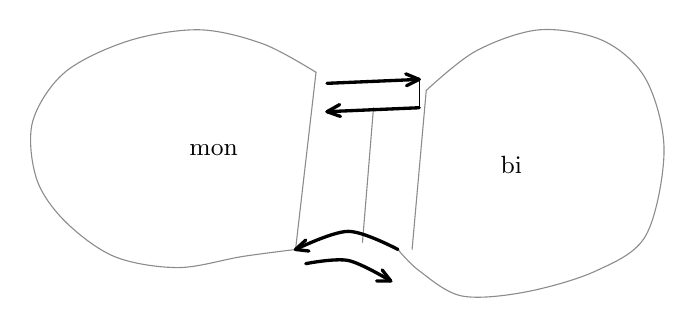
\begin{tikzpicture}[x=1mm,y=1mm,line cap=round,line join=round,font=\scriptsize]
\draw[pencil] plot[smooth, tension=0.55] coordinates {(47.2,-11.7) (40.5,-8.1) (32.4,-6.3) (23.4,-7.7) (15.3,-11.7) (11.2,-18) (11.7,-25.2) (15.3,-30.6) (21.6,-35.1) (29.7,-36.5) (37.8,-35.1) (44.6,-34.2)};
\draw[pencil] plot[smooth, tension=0.55] coordinates {(61.2,-14) (67.5,-9) (75.6,-6.3) (83.7,-7.7) (89.1,-12.6) (91.4,-21.6) (89.1,-32.4) (82.8,-36.9) (73.8,-39.6) (65.7,-40.1) (60.3,-36.9) (57.6,-34.2)};
\draw[pencil] (47.2,-11.7) -- (44.6,-34.2);
\draw[pencil] (54.5,-16.2) -- (53.1,-33.3);
\draw[pencil] (61.2,-14) -- (59.4,-34.2);
\draw[very thick] (48.6,-13.1) -- (60.3,-12.6);
\draw[very thick] (58.6,-11.9) -- (60.3,-12.6) -- (58.7,-13.4);
\draw (60.3,-12.6) -- (60.3,-16.2);
\draw[very thick] (60.3,-16.2) -- (48.6,-16.7);
\draw[very thick] (50.3,-17.3) -- (48.6,-16.7) -- (50.2,-15.8);
\draw[very thick] plot[smooth, tension=0.55] coordinates {(57.6,-34.2) (51.3,-31.9) (44.6,-34.2)};
\draw[very thick] (46.3,-34.4) -- (44.6,-34.2) -- (45.9,-33);
\draw[very thick] plot[smooth, tension=0.55] coordinates {(45.9,-36) (51.3,-35.6) (56.7,-38.2)};
\draw[very thick] (55.6,-36.8) -- (56.7,-38.2) -- (54.9,-38.2);
\node[inner sep=1pt] at (34.2,-21.6) {\small mon};
\node[inner sep=1pt] at (72,-23.4) {\small bi};
\end{tikzpicture}
\end{document}
